
%%%%%%%%%%%%%%%%%%%%%%%%%%%%%%%%%%%%%%%%%%%%%%%%%%%%%%%%%%%%%%%%%%%%%%%%%%%%%%%%%%%%%%%
%%%%%%%%%%%%%%%%%%%%%%%%%%%%%%%%%%%%%%%%%%%%%%%%%%%%%%%%%%%%%%%%%%%%%%%%%%%%%%%%%%%%%%%
% 
% This top part of the document is called the 'preamble'.  Modify it with caution!
%
% The real document starts below where it says 'The main document starts here'.

\documentclass[12pt]{article}

\usepackage{amssymb,amsmath,amsthm}
\usepackage[top=1in, bottom=1in, left=1.25in, right=1.25in]{geometry}
\usepackage{fancyhdr}
\usepackage{enumerate}
\usepackage{listings}
\usepackage{graphicx}
\usepackage{float}
\usepackage{multicol}
% Comment the following line to use TeX's default font of Computer Modern.
\usepackage{times,txfonts}
\usepackage{mwe}
\usepackage{caption}
\usepackage{subcaption}
\usepackage{svg}





\makeatletter
\renewcommand*\env@matrix[1][*\c@MaxMatrixCols c]{%
  \hskip -\arraycolsep
  \let\@ifnextchar\new@ifnextchar
  \array{#1}}
\makeatother

\newtheoremstyle{homework}% name of the style to be used
  {18pt}% measure of space to leave above the theorem. E.g.: 3pt
  {12pt}% measure of space to leave below the theorem. E.g.: 3pt
  {}% name of font to use in the body of the theorem
  {}% measure of space to indent
  {\bfseries}% name of head font
  {:}% punctuation between head and body
  {2ex}% space after theorem head; " " = normal interword space
  {}% Manually specify head
\theoremstyle{homework} 

% Set up an Exercise environment and a Solution label.
\newtheorem*{exercisecore}{Exercise \@currentlabel}
\newenvironment{exercise}[1]
{\def\@currentlabel{#1}\exercisecore}
{\endexercisecore}

\newcommand{\localhead}[1]{\par\smallskip\noindent\textbf{#1}\nobreak\\}%
\newcommand\solution{\localhead{Solution:}}

%%%%%%%%%%%%%%%%%%%%%%%%%%%%%%%%%%%%%%%%%%%%%%%%%%%%%%%%%%%%%%%%%%%%%%%%
%
% Stuff for getting the name/document date/title across the header
\makeatletter
\RequirePackage{fancyhdr}
\pagestyle{fancy}
\fancyfoot[C]{\ifnum \value{page} > 1\relax\thepage\fi}
\fancyhead[L]{\ifx\@doclabel\@empty\else\@doclabel\fi}
\fancyhead[C]{\ifx\@docdate\@empty\else\@docdate\fi}
\fancyhead[R]{\ifx\@docauthor\@empty\else\@docauthor\fi}
\headheight 15pt

\def\doclabel#1{\gdef\@doclabel{#1}}
\doclabel{Use {\tt\textbackslash doclabel\{MY LABEL\}}.}
\def\docdate#1{\gdef\@docdate{#1}}
\docdate{Use {\tt\textbackslash docdate\{MY DATE\}}.}
\def\docauthor#1{\gdef\@docauthor{#1}}
\docauthor{Use {\tt\textbackslash docauthor\{MY NAME\}}.}
\makeatother



\usepackage{mathabx}





% Shortcuts for blackboard bold number sets (reals, integers, etc.)
\newcommand{\Reals}{\ensuremath{\mathbb R}}
\newcommand{\Nats}{\ensuremath{\mathbb N}}
\newcommand{\Ints}{\ensuremath{\mathbb Z}}
\newcommand{\Rats}{\ensuremath{\mathbb Q}}
\newcommand{\Cplx}{\ensuremath{\mathbb C}}
%% Some equivalents that some people may prefer.
\let\RR\Reals
\let\NN\Nats
\let\II\Ints
\let\CC\Cplx

%%%%%%%%%%%%%%%%%%%%%%%%%%%%%%%%%%%%%%%%%%%%%%%%%%%%%%%%%%%%%%%%%%%%%%%%%%%%%%%%%%%%%%%
%%%%%%%%%%%%%%%%%%%%%%%%%%%%%%%%%%%%%%%%%%%%%%%%%%%%%%%%%%%%%%%%%%%%%%%%%%%%%%%%%%%%%%%
% 
% The main document start here.

% The following commands set up the material that appears in the header.
\doclabel{Math 614: Homework 9}
\docauthor{Stefano Fochesatto}
\docdate{\today}

\begin{document}


\begin{exercise}{P22} Consider the graph of five web pages a, b, c, d, e, shown below, where each page links to some of the other pages as show. The goal 
  of this problem, is to comput the Google PageRank of the pages., In factm, this proble, ios about the essential idea which 
  created Google, only about 25 years ago. 
  \begin{figure}[H]
    \begin{center}
      \caption{P22 graph}
       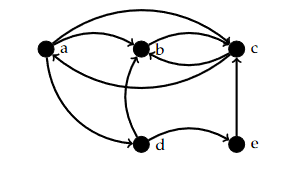
\includegraphics[width=.90\textwidth]{fig1.png}
    \end{center}
  \end{figure}
\begin{enumerate}
  \item[a.] Start by asking Google to document itself. Go to Google Scholar and search for 'pagerank citation ranking'. The firt lin, the one with highest PageRank, will be 
  a technical prepring by Page, Brin Motwani, an Winograd; it has more tha 150000 citations., Download the 17 page PDF and read it. It decrinbes a simpler time, The main ideas are about a 
  web as a directed graph, as in the example shoen above, that the limmiting probability that a ceraint random web surfer visits any partivular page is its PageRank, an finally that a 
  asearch engine should report results in the Page Rank order. We can regard PageRank as simply an eigenvector of a certina matrix $A$, a  transition probability matrix for a Markov chain. To 
  build $A$ we will start with the adjacency matrix $G$ of the web. Were is how to dtart with a web as directred graph and construct $G$,$A$ and the eigen vector of PageRank values: \\
  Let $W$ be a connecte, direcred grpha of $n$ webpages, Index the pages 1 through n. Let $G$, be the $nxn$ connectivity matrix $W$ that is, 
  \begin{equation*}
    
  \end{equation*}  
  Th=e number of nonzeroes in $G$ is the total number of hyperlinks in $W$. Let $c_j$ be the columns sums of $G$;
  \begin{equation*}
    c_j = \sum_{i = 1}^n g_{ij}
  \end{equation*}
Tghe value of $c_j$ gives the outdegreee of the $jth$ page. Let $p$ be the fraction of the time that the random walk follows some link, 
so $1-p$j is the gracion of time that an arbitratry page is chose. Define $\sigma = (1 - p)/n$.Now let $A$ be the $nxn$
 matric whose entris are, 
 \begin{equation*}
   a_{ij} = \dfrac{pg_{ij}}c_{j} + \sigma
 \end{equation*}
 The matrix $A$ is the transition probability matrix of the random-surfer Markov chain. An old theorem says the larges eigenvalus of $A$ is wqual to on 
 and the corresponding eigen vector, which satisfies
 \begin{equation*}
   Ax = x
 \end{equation*}
 is uniq1ue up to a scaling factor, and has positive entris, Choose the scaling so that,
 \begin{equation*}
   1 = \sum_{i = 1}^n x_i
 \end{equation*}
 the entris of $x$ are the Page Ranks of webpages in $W$.\\
 For a realsitive web, $G$ is huge and sparse because mose pairs of webpages are not connecred by a single link. Google suggests $p = .85$.
 Matrix $A$ is not spare because mose entris are equal to the small constant $\sigma > 0$. The 'old' Perron=Frobenius Theorem says that if all entries ina matrix
 are positie then all the entries of the eigenvectro associated to the larges eigenvalue can ve chose to be posoitb.


 \vspace{1in}

 \item{b.} Folling my descriptino of the process, compute $G$ for the web shown above. \\
 \solution From the passage above we know that $G$ is the adjacency matrix for the figure 1. Building the adjacency matrix we get, 
 \begin{equation*}
   \begin{bmatrix}
     0 & 0 & 1 & 0 & 0\\
     1 &0 &1 &1 &0\\
     1&1 & 0& 0&1\\
     1&0 &0 &0 &0\\ 
     0&0 &0 &1 &0
   \end{bmatrix}
 \end{equation*}
 \vspace{1in}


 \item[c.] Continueing from my description, build $A$ from $G$ using $p = .85$ as sugestged. Finnaly, use Matlabs eig to compute the PageRanks. Which page gets the highest PageRank?
 explain in intuative terms.\\
 \solution The following Matlab script computes $A$ from $G$, and uses the eig() function to compute the PageRanks




\end{enumerate}

  \end{exercise}













\end{document}




















